\chapter{Quantum Physics Basics}

In this chapter, we will study the laws of nature at very small scales.

We start by reviewing classical concepts like particles or waves, and then see how they break down when being applied to the microscopic world. For those observations that could not be explained with classical physics, we need \emph{quantum physics}. The theory of quantum physics is very deep and profound, so surely way beyond the scope of our course. What we will study in this A-Level course are merely four tips of an enormous iceberg, namely

\begin{compactenum}
	\item[-] photon theory / photoelectric effect
	
	\item[-] matter waves / electron diffraction
	
	\item[-] electron energy levels / atomic spectra
	
	\item[-] band theory / electrical conductivity of solids
\end{compactenum}

\subsection{classical theories}

in classical physics, both particle models and the wave models have been very useful

though both being successful, the two model are distinct in many aspects

to understand a phenomenon, we take either the particle picture or the wave picture

it seems that there is no way particle models would reconcile with wave models, or is it not?

\subsection{particle models}

in particle model, any system is considered to consist of particles governed by \emph{Newtonian mechanics}, physical properties of this system are predicted by studying behaviour of particles

\cmt areas of science where particle models are used to interpret and make predictions include:

\begin{compactenum}
	\item[-] \emph{electricity}: electric current formed by motion of charge carriers
	
	\item[-] \emph{ideal gas}: pressure caused by collisions of gas molecules
	
	\item[-] \emph{solid}: elasticity due to interaction between solid atoms
	
	\item[-] \emph{radioactivity}: decay interpreted as the emission of $\alpha$-/$\beta$-particles from the nucleus
	
	\item[-] \emph{chemistry}: chemical reactions due to exchange of electrons between atoms and molecules
	
	\item[-] $\cdots$
\end{compactenum}

\subsection{wave models}

in the wave picture, energy is transferred via the vibration of medium or force fields

\cmt phenomena that can be explained in terms of wave models include:

\begin{compactenum}
	\item[-] \emph{water waves}: variation in the vertical displacement of water surface
	
	\item[-] \emph{propagation of sound}: variation in the pressure and density of medium
	
	\item[-] \emph{light}: variation of electric and magnetic fields
	
	\item[-] $\cdots$
\end{compactenum}

\cmt a key feature that makes waves distinct from particles is that waves can \emph{superpose}

when two or more waves meet, they add up or cancel out to give a resultant wave

this gives rise to the characteristic properties of waves:

\begin{compactenum}
	\item[-] \emph{interference}: waves superpose to form a resultant wave of greater or lower amplitude
	
	\item[-] \emph{diffraction}: bending of waves around obstacles, or spreading out of waves through slits
\end{compactenum}



\subsection{history of light}

efforts to understand the nature of light can be traced all the way back to ancient Greeks 

we are not going to examine the ideas of early thinkers well over 3,000 years ago

let's skip a couple of years and jump to the ideas developed since the Scientific Revolution


\cmt particle theory of light (\emph{Issac Newton}, 1671)

key idea: light rays is comprised of a stream of massless particles called \emph{corpuscles}

\begin{compactitem}
	\item[--] explains straight-line propagation
	
	\item[--] explains reflection and refraction
	
	\item[--] explains colours of light seen in dispersion in prism (corpuscles have different colours)
\end{compactitem}

the problems with the particle model include:

\begin{compactitem}
	\item[--] does not agree with observations on refraction
	
	\item[--] cannot predict the interference and diffraction of light
\end{compactitem}

\cmt wave theory of light (\emph{Christian Huygens}, 1678)

key idea: light is a wave that transfers energy within a medium known as \emph{aether}

\begin{compactitem}
	\item[--] follows laws of reflection and refraction
	
	\item[--] explains colours of light (light have different wavelengths)
	
	\item[--] explains interference (Thomas Young's double slit experiment)
	
	\item[--] explains diffraction (Poisson spot experiment)
\end{compactitem}

only problem is that aether, the medium in which light lives, was not experimentally found

\cmt electromagnetic theory (\emph{James Maxwell}, 1865)

key idea: light is an \emph{electromagnetic wave}
\footnote{\emph{Maxwell's equations} fully describe the behaviour of electric and magnetic fields. Based on the four equations that Maxwell established, he found the vibration of electric and magnetic field can propagate in space as a classical wave. The speed of electromagnetic wave is given by
	
	{
		
		\centering
		
		$c=\frac{1}{\sqrt{\epsilon_0\mu_0}}=\frac{1}{\sqrt{8.85\times10^{-12}\times4\pi\times10^{-7}}} = 3.00 \times 10^8 \mps$,
		
	}
	
	\noindent which is the same as speed of light. This gave Maxwell the intuition that light is an electromagnetic wave.}

\begin{compactitem}
	\item[--] electric and magnetic fields travel through space in the form of waves at speed of light
	
	\item[--] propagation of electromagnetic wave does not require medium, hence no need for aether
	
\end{compactitem}

all behaviour of light known at that time could be explained with Maxwell's theory

so scientists were convinced that light travelled through space as an electromagnetic wave


\subsection{photon theory}


\subsection{photoelectric effect}\label{ch-photoelectricity}

electromagnetic radiation incident upon a metal can cause emission of electrons from the metal surface, this is called \keypoint{photoelectric effect}\index{photoelectric effect}, 
\footnote{Photoelectric effect was first observed in 1887 by \emph{Heinrich Hertz}, who found electrodes illuminated with ultraviolet light create electric sparks. In school labs, one can shine ultraviolet radiation from a mercury lamp onto a zinc plate to cause photo-emission.}
emitted electrons are called \keypoint{photoelectrons}

simply put, conduction electrons in metal gain additional energy by absorbing the incoming radiation, if this energy is sufficient for electrons to overcome the electrostatic attraction from the positive metal ions, they break free from the metal surface.

\begin{figure}
	\centering
	\begin{tikzpicture}[scale=1.2]
	\tikzset{photon/.style={thick, decorate, purple, decoration={snake,segment length=0.8cm,amplitude=4pt}}}
	\draw[thick] (-3,-1) -- (-1.5,1) -- (3,1) -- (1.5,-1) -- cycle;
	\foreach \r in {-4,-3.5,-3} \draw[photon,->] (\r,\r+6) --++ (2.7,-2.5);
	\foreach \r in {-0.5,0,0.5} \draw[blue,thick,->] (\r+0.5,-\r) --++ (3,2.5);
	\shade [ball color = green] (0,0) circle (0.1);
	\shade [ball color = green] (-1,0.5) circle (0.1);
	\shade [ball color = green] (0.8,-0.2) circle (0.1);
	\shade [ball color = green] (0.9,0.7) circle (0.1);
	\shade [ball color = green] (1,-0.7) circle (0.1);
	\shade [ball color = green] (-0.5,-0.4) circle (0.1);
	\shade [ball color = green] (-1.9,-0.6) circle (0.1);
	\draw (-1,-0.8) --++ (-1.2,-0.8) node[left]{metal plate};
	\node[twoline] at (-1.2,2.6) {electromagnetic\\radiation};
	\node[twoline] at (1.5,2.7) {electrons\\released};
	\end{tikzpicture}
\end{figure}


\cmt some detailed experimental observations on the photoelectric effect are:

\begin{compactitem}
	\item[--] there exists a minimum \keypoint{threshold frequency}\index{photoelectric effect!threshold frequency} $f_0$ for incident radiation
	
	when $f<f_0$, no electrons released from metal surface
	
	\item[--] emission of electrons is immediate when radiation is incident as long as $f>f_0$
	
	even low-intensity light is effective
	
	\item[--] increasing intensity has no effect on energies of electrons
	
	\item[--] increasing intensity of incident light causes number of photoelectrons emitted to increase
	
	\item[--] increasing radiation frequency increases electron energies
\end{compactitem}

\cmt wave theory of light fails to explain any of these properties, according to wave model:

\begin{compactitem}
	
	\item[--] electrons could gradually build up energies by absorbing wave energy over time
	
	so radiation at any frequency should all work 
	
	
	\item[--] need very intense light to have immediate effect
	
	\item[--] greater intensity mean higher energy, electrons released should have greater K.E.
	
	\item[--] varying frequency of radiation should have no effect on energy of electrons released
\end{compactitem}

photoelectric effect sees the breakdown of the wave model, some new ideas are needed!

\newpage
\section{The Photo-electric Effect}
When electromagnetic radiation of high enough frequency falls on a metal surface, electrons are emitted from the surface.
For most metals, ultraviolet is needed. For some (including sodium, potassium, caesium), light towards the violet end of the spectrum) will release electrons.

 
\subsection{Demonstrating the Photo-electric Effect}

Either using a zinc plate with a gold leaf electroscope (or a coulombmeter)
\begin{figure*}
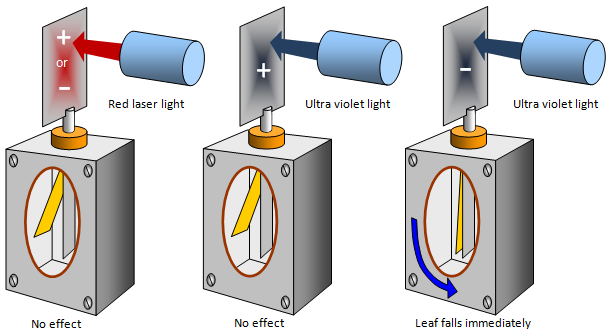
\includegraphics[]{photoelec.png}
\caption{Photoelectric effect demonstrated with electroscope}
\end{figure*}
\begin{itemize}
\item Clean a zinc plate with fine emery paper or steel wool.
\item Attach the plate to the top disc on a gold leaf electroscope, so there is good electrical contact.
\item Charge the zinc plate and inner assembly of the electroscope negatively, e.g. by rubbing the zinc plate with a polythene rod which has been rubbed with wool or fur. The leaf should now be raised, because the leaf and the back plate are both charged negatively and repel each other. The leaf should temporarily rise further if the charged polythene rod is brought near the zinc plate.
\item Place an ultraviolet lamp near the zinc plate. Switch it on. The leaf should be seen to fall. [Safety note: Don't look at the ultraviolet lamp (when it's turned on!)] Clearly the plate (and inner assembly of electroscope) is losing charge.
\item Repeat the procedure, but charging the zinc plate and inner assembly of the electroscope positively, e.g. by rubbing the plate with a charged perspex rod. This time the ultraviolet does not affect the leaf. Charge is not lost.
     \end{itemize}
The simplest explanation is the correct one\ldots The ultraviolet causes electrons to be emitted from the zinc plate. If the plate is charged positively, the electrons are attracted back again. If the plate is charged negatively the emitted electrons are repelled and lost from the plate for ever. 

\subsection{Photo-electric Puzzles}
Before 1905, the energy of a beam of light was thought of as distributed uniformly across broad wavefronts. Calculations showed that it should take some time before an electron in a metal surface could absorb enough energy from the light to escape from the surface. Yet emission is observed as soon as the light falls on the surface.
Another puzzle was why, for a given surface, we find that light of frequency below a certain value (the threshold frequency) causes no electron emission at all.
Einstein's theory of the photo-electric effect solves both these problems\ldots

\subsection{Einstein's Photo-electric Equation}
Although the free electrons in a metal have no allegiance to particular atoms, there are forces `bonding' them to the lattice of ions as a whole. In order to escape from the metal an electron has to do work against these forces. Some have to do more work than others, but there is a certain minimum quantity of work to be done, so no electron can escape unless it is given a certain minimum energy.
The work function, $\phi$, of a metal is the minimum energy needed by an electron in order to escape from the surface. 
Einstein's key idea was that any electron which leaves the surface is ejected by the action of a single photon. Photons don't co-operate in the process.
Recall that a photon of light of frequency $f$ has energy $= hf$. 
Suppose that a photon gives its energy $hf$ to an electron, and that the electron is able to escape. The minimum energy used in escaping is $\phi$, so the maximum kinetic energy the escaped electron can have is what's left over of the photon's energy. So we have the simple equation:
\[ E_{Kinetic} =hf - \phi \]


This assumes that the photon energy is greater than (or equal to) the work function; in other words that  $hf>\phi$ or $f=\phi/h$.
If  $f < \phi/h$, the photon energy will be less than the work function so no electrons at all can escape - a simple explanation of the phenomenon of threshold frequency.
 
The threshold frequency, $f_0$, for a metal is the minimum frequency of electromagnetic radiation needed to produce electron emission from the surface.
From the argument just given, 
\[f_{0} =  \phi/ h.\]
This relationship can also be deduced from Einstein's equation; At the threshold frequency even the most energetic electron will only just manage to escape, so $KE_{max} =  0$, and therefore     $f0 = \phi/h$.
Provided that the light is above the threshold frequency, as soon as it falls on the metal surface electrons will start to be emitted, as emission results from individual photon `hits', and is not a cumulative process as supposed before Einstein.

\subsection{Experimental test of Einstein's Equation}

We use the arrangement with the vacuum photocell shown below  for demonstrating the photoelectric effect.

\begin{figure}
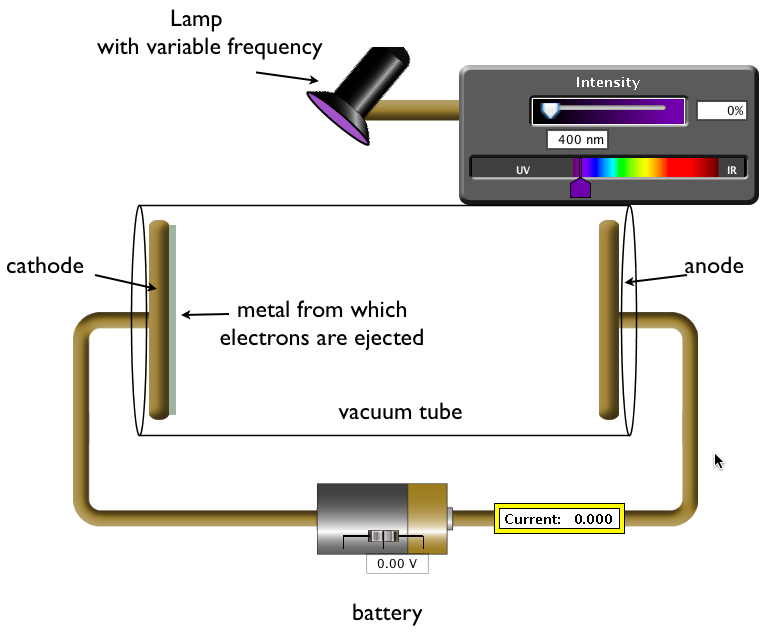
\includegraphics[]{vaccell.png}
\caption{Photoelectric effect with vacuum cell. Note: Picture comes from the fantastic simulation at Phet.}
\end{figure}

\begin{itemize}
\item Use white light with a coloured filter, or a light emitting diode, to illuminate the metal surface with approximately monochromatic light. [Its wavelength can be found using a diffraction grating, hence its frequency, using $f = c / \lambda$ .]
\item Increase the p.d. between the collecting electrode and the metal surface until the current drops to zero. 
At this point the p.d. is called the stopping voltage, $V_{stop}$, because it stops all emitted electrons, even those with the most K.E., from reaching the collector electrode.

\item The maximum K.E. of the emitted electrons is simply given by \sidenote{How do we justify this? Because of the applied voltage, emitted electrons are subject to repulsion by the positive collector electrode and attraction by the emitting surface, hence to a resultant force towards the emitting surface. The electrons therefore get slower and slower as they cross the gap. When the stopping voltage is applied, even the most energetic of emitted electrons have no K.E. left when they have made it across the gap. The K.E. lost is equal to the P.E. gained for these electrons. That's what the equation states.
It is just like finding the K.E. of a ball thrown upwards in the Earth's gravitational field by measuring the its maximum height, and using the energy conservation equation  K.E. lost = mgh}

\[ E_{k} = V_{Stop} \times 1.6 \times 10^{-19} \]


\item Repeat the process using two or three more frequencies of light.
\item Plot a graph of $KE_{max}$ against frequency, $f$. If Einstein's equation is correct it should have a positive slope equal to $h$ and a negative intercept, equal to $ \phi $. We can see this by comparing Einstein's equation with $y = mx + c$.
\begin{align*}
E &= &hf &-& \phi \\
y &= &mx& + &c
\end{align*}
\end{itemize}

A sample graph is presented below.

\begin{figure}
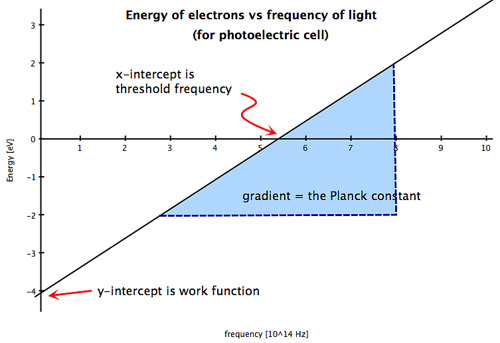
\includegraphics[scale=.6]{photograp.jpg}
\caption{A graph of Frequency vs Kinetic energy}
\end{figure}

It is useful practice to find from the graph:
\begin{itemize}
\item a value of Planck's constant,
\item the threshold frequency for the metal,
\item the threshold wavelength for the metal
\item the work function for the metal
\end{itemize} \sidenote{In practice it is difficult to obtain a good value for h using a commercially available vacuum photocell. Slight impurities on the metal surface (e.g. a thin oxide film), and unwanted electron emission from the collector electrode, both affect the stopping voltage. The first convincing verification of Einstein's photo-electric equation, leading to an accurate value of the Planck constant was completed in 1916 by R.A. Millikan, working in the United States. The secret of his success was a remotely operated knife working in the vacuum to skim off surface layers from the caesium surface as they became contaminated.}
 
\subsection{Effect of changing the Light Intensity}
If we bring a monochromatic light source towards a surface we increase the light energy falling on the surface, per $m^2$, per $s$. We are said to be increasing the intensity of the light. Clearly we can apply the same idea to ultraviolet or any other electromagnetic radiation. We find that:
\begin{enumerate}
\item For light or ultraviolet of a given frequency, changing the intensity has no effect on the maximum K.E. of the emitted electrons. This is exactly what Einstein's theory predicts. The energy given to individual electrons comes from individual photons, and a photon's energy, $hf$, depends only on the frequency (or, equivalently, the wavelength) of the radiation. It doesn't, then, depend on its intensity (provided we don't change the frequency).

\item For light or ultraviolet of a given frequency, increasing the intensity increases the number of electrons emitted per second.
\end{enumerate}
Again, this is just what we'd expect from Einstein's theory. Increasing the intensity means increasing the number of photons arriving at the surface, per m2, per s.  Naturally this means that more electrons will be emitted. \sidenote{Each identical photon has the same probability of emitting an electron.} 
	We can show the effect with the same vacuum photocell arrangement used for demonstrating the photoelectric effect. Note that the polarity of the power supply is arranged to encourage electrons to cross the gap.
    \begin{itemize}
    \item Use a monochromatic light source to illuminate the caesium surface.
\item Check that increasing the p.d. does not affect the current, I. This means that all the electrons emitted per second are being collected.
\item Bring the light source closer and observe the effect on I.
\item I is the charge flowing per second, so the number of electrons emitted per second is I/e in which e is the charge on each electron.
 \end{itemize}





\subsection{photon theory}

photoelectric effect was explained by \emph{Albert Einstein} in 1905
\footnote{Albert Einstein was awarded the Nobel Prize in physics in 1921 for `his discovery of the law of the photoelectric effect'. This discovery led to the quantum revolution of modern physics.}

Einstein's revolutionary idea: when radiation delivers energy to matter, the transfer of energy is not continuous but carried in \emph{discrete} packets, called \emph{photons}

\begin{ilight}
	a \keypoint{photon}\index{photon} is a packet (\emph{quanta}) of electromagnetic energy
\end{ilight}

\cmt energy of one photon is given by: \begin{empheq}[box=\tcbhighmath]{equation*}{E=hf}\end{empheq}, where $h=6.63\times10^{-34} \text{ J s}$ is the \keypoint{Planck constant}\index{Planck constant}

since $E \propto f$, higher/lower radiation frequency means greater/smaller photon energies

\cmt wave equation $c=\lambda f$ relates frequency $f$ of an electromagnetic wave to its wavelength $\lambda$

so energy of one photon is also given by: \begin{empheq}[box=\tcbhighmath]{equation*}{E=\frac{hc}{\lambda}}\end{empheq}

since $E \propto \frac{1}{\lambda}$, longer/shorter wavelength means lower/greater photon energies

\cmt the equation $E=hf$, or $E=\frac{hc}{\lambda}$,  relates a particle property with a wave property

$E$ is the energy of one photon, treated like a single particle

but $f$ and $\lambda$ are both introduced to describe a wave, not a particle

\cmt intensity of a beam of radiation is: $I = \frac{P}{A}$

total energy incident on a given area per unit time determines the radiation intensity

so intensity depends on the product of the number of photons arriving per unit time and energy of each photon: $ \tcbhighmath{I \propto nhf}$, or more precisely, \begin{empheq}[box=\tcbhighmath]{equation*}I = \frac{nhf}{A}\end{empheq}

\cmt when considering energy of a photon, \keypoint{electronvolt} is a useful energy unit

one electronvolt (1 eV) is work needed to make an electron travel through a p.d. of 1 V

conversion between electronvolt and joule is: \begin{empheq}[box=\tcbhighmath]{equation*}{1 \text{ eV} = 1.60\times10^{-19} \text{ J}}\end{empheq}

\example{A laser emits red light of 650 nm at a power rating of 2.0 mW. (a) What is the energy carried by one photon? (b) How many photons are emitted per second?}\label{ex-redlaser}

\begin{soln}
    
energy of one photon: $E = \frac{hc}{\lambda} = \frac{6.63\times10^{-34}\times3.0\times10^8}{650 \times10^{-9}} \approx 3.06\times10^{-19} \text{ J}$

\eqyskip number of photons: $N = \frac{\text{total energy output from laser}}{\text{energy of one photon}} = \frac{2.0\times10^{-3}}{3.06\times10^{-19}} \approx 6.54\times10^{15}$ \end{soln}

\question{Calculate the energy, in eV, of a photon of light of wavelength 440 nm.}

\question{If the light source in Example \ref{ex-redlaser} is replaced by a green laser with the same power output, how does the number of emitted photons per unit time change?}




\subsection{photoelectric effect explained}

from the viewpoint of photon theory, photoelectric effect can be explained easily

to release an electron from metal, it requires a minimum energy $\Phi$, called the \keypoint{work function}\index{photoelectric effect!work function}, for the electron to overcome attraction due to metal ions to escape from metal surface

as radiation shines upon metal, photon energies are absorbed by electrons

since photon energies are \emph{discrete}, or \emph{quantised}, the absorption is sort of all or nothing

if photon energy is greater than $\Phi$, electrons break free from metal

excess energy, if any, would become kinetic energy of the free electron

this is summarised in \keypoint{Einstein's photoelectric equation}\index{photoelectric effect!photoelectric equation}: 
\begin{empheq}[box=\tcbhighmath]{equation*}{hf = \Phi + E_{k,\tmax}}\end{empheq}

\cmt note that we are talking about \emph{maximum} K.E. of emitted electrons

electron emitted from the \emph{surface} would have greatest K.E.

for electrons to be released from \emph{below} the surface, they require more energy than work function, so less K.E. than maximum value

\cmt at critical condition, incoming photon has just enough energy to release electron

so at threshold frequency\index{photoelectric effect!threshold frequency} $f_0$, photon energy equals work function: \begin{empheq}[box=\tcbhighmath]{equation*}{hf_0 = \Phi}\end{empheq}

\cmt experimental observations mentioned in \S\ref{ch-photoelectricity} can now be understood

\begin{compactitem}
	
	\item[--] below threshold frequency $f_0$, not enough photon energy available to electron to overcome work function, so no effect for $f<f_0$
	
	\item[--] interaction between photon and electron is \emph{one-to-one}, so no time delay
	
	\item[--] greater radiation intensity means more photons per unit time, so more electrons released
	
	\item[--] greater frequency means higher photon energy, so greater K.E. for emitted electron
	
\end{compactitem}


\example{Given that work function energy of gold is 4.9 eV. Find the longest wavelength of electromagnetic wave that could release electrons from gold.}

\begin{soln}
    
 threshold frequency: $f_0 = \frac{\Phi}{h} = \frac{4.9\times1.60\times10^{-19}}{6.63\times10^{-34}} \approx 1.18\times10^{18} \text{ Hz}$

threshold wavelength: $\lambda_0 = \frac{c}{f_0} = \frac{3.00\times10^8}{1.18\times10^{15}} \approx 2.54\times10^{-7} \text{ m} \,$ (ultraviolet light) \end{soln}

\question{Sodium has a work function of $3.8\times 10^{-19} \text{ J}$. (a) Find the threshold frequecy for sodium. (b) If a light of 500 nm is incident on sodium, determine whether electrons can be emitted from the surface.}

\question{When electromagnetic radiation of wavelength 1200 nm is incident on a metal surface, the maximum kinetic energy of the electrons released is found to be $5.4\times10^{-20} \text{ J}$. What is the work function of this metal?}

\question{When a beam of light of a particular frequency and intensity is shone onto a metal surface, electrons are released. If another beam of light of same intensity but higher frequency is used, what is the effect on the rate of emission of electrons from this surface?}

\subsection*{measurement of the Planck constant and work function energy}

when radiation with different frequencies is incident onto a metal, we measure maximum K.E. of the electrons emitted from the surface, a set of readings $(f, E_{k,\tmax})$ can be found

note that the photoelectric equation can be rearranged as: $ E_{k,\tmax} = hf - \Phi$

\begin{marginfigure}
	\vspace*{-12pt}
	\centering
	\begin{tikzpicture}[scale=1.2]
	\draw[thick,->] (0,-1.6) -- (0,2.4) node[left]{$E_{k,\tmax}$};
	\draw[thick,->] (0,0) -- (4,0) node[below]{$f$};
	\draw[thick,blue, dashed] (0,-1.2) -- ++(1.6,1.6);
	\draw[thick,blue] (1.6,.4) -- ++(1.8,1.8);	
	\node[left] at (0,-1.2) {$-\Phi$};
	\node[left] at (0,0) {$0$};
	\node[below right] at (1.2,0) {$f_0$};
	\end{tikzpicture}
	\vspace*{-12pt}
\end{marginfigure}

if we plot a graph of $ E_{k,\tmax} $ against $f$, data points shall fall on a straight line

information about the Planck constant $h$, threshold frequency $f_0$, work function $\Phi$ can all be computed with the best-fit line

\begin{compactitem}
	\item[--] $\text{gradient} = h$
	
	\item[--] $y\text{-intercept} = -\Phi$
	
	\item[--] $x\text{-intercept} = \frac{\Phi}{h} = f_0$	
\end{compactitem}

\question{If a different metal with a greater work function energy is used, describe the change for the line that shows the variation with $f$ of $E_{k,\tmax}$ for this metal.}

\question{Electromagnetic adiation is incident upon a metal plate. The graph shows how maximum kinetic energy $E_k$ of emitted electrons varies with frequency $f$ of the radiation. Use the graph to find (a) the threshold frequency, (b) a value of Planck constant.}
	
\begin{center}
	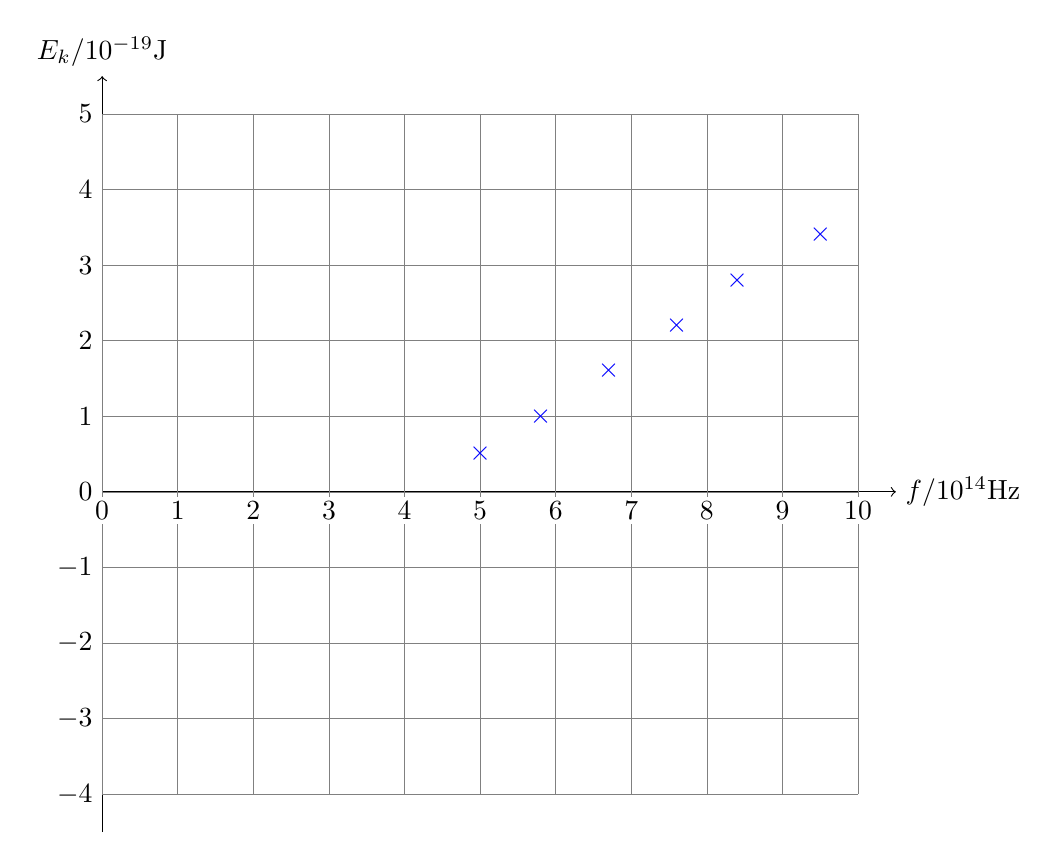
\begin{tikzpicture}[scale=0.96]
		\draw[->] (0,-4.5) -- (0,5.5) node[above]{$E_k$/10$^{-19}$J};
		\draw[->] (0,0) -- (10.5,0) node[right]{$f$/10$^{14}$Hz};
		\draw[step=1, gray, very thin] (0,-4) grid (10,5);
		\foreach \x in {0,1,...,10} {
			\draw[white,fill] (\x-0.2,-0.42) rectangle (\x+0.2,-0.08);
			\node[below] at (\x,0) {$\x$};
		}
		\foreach \y in {-4,-3,...,5} \node[left] at (0,\y) {$\y$};
		\node[blue] at (5.0,0.5) {$\times$};
		\node[blue] at (5.8,1.0) {$\times$};
		\node[blue] at (6.7,1.6) {$\times$};
		\node[blue] at (7.6,2.2) {$\times$};
		\node[blue] at (8.4,2.8) {$\times$};
		\node[blue] at (9.5,3.4) {$\times$};
	\end{tikzpicture}
\end{center}
	


\subsection{photon momentum}

in photoelectric effect, photons can knock electrons out of a metal, this suggests that photons could have \emph{momentum}, even though they do not have mass

earliest experimental evidence of photon momentum was came from \emph{Arthur Compton} in 1923, who studied the scattering of X-ray photons by electrons in substances\footnote{Arthur Compton was awarded the Nobel Physics Prize in 1929 for the discovery of this scattering effect, now known as \emph{Compton scattering}.}

it can be shown\footnote{This derives from Einstein's theory of \emph{special relativity}, which states that energy and momentum are related by the equation: $E^2 = m_0^2 c^4 + p^2 c^2$. Photons have zero rest mass, i.e., $m_0=0$. This relativistic relation becomes $E=pc$ for photons. Now recall photon energy is given by $E=hf$. Rearrange the terms, we can show: $p = \frac{hf}{c} = \frac{h}{\lambda}$.} that photon momentum is given by: \begin{empheq}[box=\tcbhighmath]{equation*}{p = \frac{h}{\lambda}}\end{empheq}

\cmt photon momentum a \emph{relativistic} momentum, as photons move at speed of light

definition for classical momentum $p=mv$ does not apply for photons

\cmt due to exchange of momentum, electromagnetic wave can exert \emph{radiation pressure}

forces generated by radiation pressure are negligible under everyday circumstances, but they could have noticeable effects on spacecraft in outer space and comet tails

\example{A beam of light has wavelength 600 nm, cross-sectional area $0.16 \text{ cm}^2$ and power 5.0 mW. The beam is normally incident onto a surface and is completely absorbed. Calculate, for a time of 1.0 s, (a) the number of photons incident onto the surface, (b) the change of total momentum of the photons, (c) the light pressure on the surface.}

\begin{soln}
    
 energy of one photon: $E= \frac{hc}{\lambda} = \frac{6.63\times10^{-34} \times 3.0\times10^8}{600\times10^{-9}} \approx 3.32 \times 10^{-19} \text{ J}$ 1.5083


number of photons arriving in 1.0 s: $N = \frac{5.0\times10^{-3} \times 1.0}{3.32 \times 10^{-19}} \approx 1.51\times10^{16}$

momentum for one photon: $p = \frac{h}{\lambda} = \frac{6.63\times10^{-34}}{600\times10^{-9}} \approx 1.11 \times 10^{-27} \text{ kg m s}^{-1}$

change of total momentum: $\Delta P = Np = 1.51\times10^{16} \times 1.11 \times 10^{-27} \approx 1.67 \times 10^{-11} \text{ kg m s}^{-1}$

average force due to these photons: $F = \frac{\Delta P}{\Delta t} = \frac{1.67 \times 10^{-11}}{1.0} \approx 1.67 \times 10^{-11} \text{ N}$

light pressure on surface: $p = \frac{F}{A} = \frac{1.67 \times 10^{-11}}{0.16 \times 10^{-4}} \approx 1.04 \times 10^{-6} \text{ Pa}$ \end{soln}

\question{A laser of power $P$ is incident normally on a spot of area $A$, show that the pressure caused by the beam can be given by: $p = \frac{P}{cA}$.}

\question{When an electron and a positron meet together, they will annihilate and produce two $\gamma$-photons: $^{\phantom{+}0}_{-1}e + ^{\phantom{+}0}_{+1}e \longrightarrow \gamma + \gamma$. Assume the electron and the positron have negligible kinetic energy before the interaction, explain why the two photons produced must move off in opposite directions with equal energies.}

\subsection{wave-particle duality}



\subsection{matter waves}

inspired by photon theory, which shows electromagnetic waves have a particulate nature, \emph{Louis de Broglie} suggested in his 1924 PhD thesis that all matter has a wave-like nature
\footnote{Louis de Broglie was awarded the 1929 Nobel Physics Prize `for his discovery of the wave nature of electrons'. \emph{Schr\"oedinger's equation} and \emph{Bohr's atomic model} was heavily influenced by ideas of de Broglie.}

wave characteristic of a particle can be represented by a wavelength

\begin{ilight}
	\keypoint{de Broglie wavelength}\index{de Broglie wavelength} of a matter particle is given by:\begin{empheq}[box=\tcbhighmath]{equation*}{\lambda = \frac{h}{p}}\end{empheq}, where $p=mv$ is the particle's momentum
\end{ilight}

\example{What is the wavelength of a human of 70 kg walking at around $2.0\mps$?}

\begin{soln}
    $\lambda = \frac{h}{mv} = \frac{6.63\times10^{-34}}{75\times 2} \approx 4.7\times 10^{-36} \text{ m}$

this wavelength is too small compared with any obstacle we encounter in everyday lives

so human bodies do not exhibit noticeable wave behaviour \end{soln} 

\example{An electron is accelerated from rest through a potential difference of 50 V. What is the de Broglie wavelength of this electron?}
\begin{soln}
K.E. of electron equals change in electric P.E., so
$\frac{1}{2}mv^2 = qV \RA v = \sqrt{\frac{2qV}{m}} = \sqrt{\frac{2\times1.60\times 10^{-19} \times 50}{9.11\times10^{-31}}} \approx 4.19\times10^6 \mps$


wavelength of electron: $\lambda = \frac{h}{mv} = \frac{6.63\times10^{-34}}{9.11\times10^{-31}\times 4.19\times10^6} \approx 1.74 \times10^{-10} \text{ m}$

this wavelength is comparable to scale of atomic spacing (also around $10^{-10}\text{ m}$)

so these electron can be \emph{diffracted} by solid crystals\end{soln}

\question{An $\alpha$-particle is moving with a kinetic energy of $2.4\times10^{-15} \text{ J}$. Find its speed, and hence find its de Broglie wavelength.}

\question{If a proton and an electron are accelerated through the same voltage, (a) how would their energy compare? (b) how would their wavelength compare?}

\subsection{electron diffraction}


wave property of electron was confirmed by \emph{Clinton Davisson} and \emph{George Thomson} in 1927

they showed experimentally electrons could be diffracted\index{electron diffraction} by metal crystals
\footnote{The Nobel Prize in Physics 1937 was awarded jointly to Clinton Davisson and George Thomson `for their experimental discovery of the diffraction of electrons by crystals'}

\begin{figure}[htp]
	\centering
	\begin{tikzpicture}[scale=1]
	\draw[gray!40,fill] (-0.5,-1) -- (-0.5,0.5) -- (0.5,1) -- (0.5,-0.5) -- cycle;
	\draw[thick,blue,->] (-3,0) -- (-.5,0);
	\draw[gray!20,fill] (5,-3) -- (5,1.5) -- (7,3) -- (7,-1.5) -- cycle;
	\draw[blue, dashed, fill=blue!50, opacity=0.3] (0,0) -- (6,1.2) [out = 0, in=0] to (6,-1.2) --cycle;
	\draw[blue, dashed, opacity=0.3] (6,1.2) [out = 180, in=180] to (6,-1.2);
	\draw[green,fill] (6,0) ellipse (0.06 and 0.12);
	\draw[green,line width=2pt] (6,0) ellipse (0.2 and 0.4);
	\draw[green,line width=2pt] (6,0) ellipse (0.35 and 0.7);
	\draw[green,line width=1.5pt] (6,0) ellipse (0.55 and 1.1);
	\draw (-0.2,-0.5) --++ (-0.5,-1) node[below,twoline]{thin\\crystal};
	\draw (5.5,-2) --++ (2,-0.6) node[below,twoline] {fluoroscent\\screen};
	\draw (6.3,0.9) --++ (2.5,1.5) node[above,twoline] {diffraction pattern\\formed on screen};
	\node[twoline] at (-1.8,0.5) {electron\\beam};
	\end{tikzpicture}
	
	\caption{electron diffraction experiment}
\end{figure}

\cmt electron diffraction experiment shows that particles do have wave-like properties

if electrons behaved like particles, we would see a round spot of \emph{uniform} distribution

but the actual pattern formed on \emph{fluorescent screen} is a set of \emph{concentric rings}

this is a typical diffraction pattern, hence proves wave properties of electrons

\cmt each metal has a different lattice structure, so each produces a different pattern

this allows investigation of structure of matter (explore arrangements of atoms, structures of complex molecules, structure of atomic nuclei, etc.) using electron diffraction

\cmt since wavelength of an electron is much shorter than visible light

this allows \emph{electron microscope} to have much higher resolving power than optical microscopes

\question{If a higher p.d. is applied to accelerate the electron beam in the electron diffraction experiment, how would the pattern change?}


\subsection{wave-particle duality}

we have seen both particle-like and wave-like behaviour in light and electrons

\begin{center}
	\begin{tabular}{|D{2.5cm}|D{5.5cm}|D{5cm}|}
		\hline
		& electromagnetic radiation & electron \\ \hline
		particle-like & photoelectric effect, & deflection in electric/magnetic \\
		behaviour & radiation 	pressure &  fields, decay, scattering \\  \hline
		wave-like behaviour & interference, diffraction, Doppler
		effect, reflection, refraction & electron diffraction \\ \hline
	\end{tabular}
\end{center}

when light/electron move through space, they behave like a wave

when light/electron interact with each other, they behave like particles

they show a two-sided nature, or a \emph{dual} nature of being both a wave and a particle, described by either particle model or wave model under different circumstances

in fact, all matter (protons, neutrons, atoms, cells, basketballs, human body, earth, etc.) has this universal dual nature, called \keypoint{wave-particle duality}\index{wave-particle duality}

wave-particle duality addresses breakdown of classical concepts like particle or wave

to fully describe the behaviour of microscopic objects, we need \emph{quantum mechanics}
\footnote{Being a central concept of quantum theory, wave-particle duality is deeply embedded into the foundations of quantum physics. In non-relativistic quantum mechanics, all information about a particle is encoded in its \emph{wave function}, whose evolution with time is described by the famous \emph{Schr\"odinger's equation}.}




\subsection{quantisation of electron energy levels}

in a simple atomic model, electrons move around the nucleus in circular orbits

but now we understand electrons have wave properties, as an electron moves in its orbit as a wave, it can superpose with itself

only orbits in which the electron can superpose constructively with itself are preferable

so electrons are only allowed to move in certain orbits in an atom

this means can only take certain values of energy, called \emph{energy levels}



\subsection{hydrogen atom \protect\piste}

theoretical explanation for electron energy levels was developed in 1913 by Danish physicist \emph{Niels Bohr} in his theory of hydrogen atom
\footnote{Niels Bohr was surely one of the greatest physicists of the 20th century. He made foundational contributions to understanding atomic structure and quantum mechanics, for which he received the Nobel Physics Prize in 1922. He was also the founder of the Institute of Theoretical Physics at the University of Copenhagen, which soon became the centre of pioneering researches on quantum theory in the world.}

let's look at the hydrogen atom -- the simplest possible atom in nature

\begin{marginfigure}
	\centering
	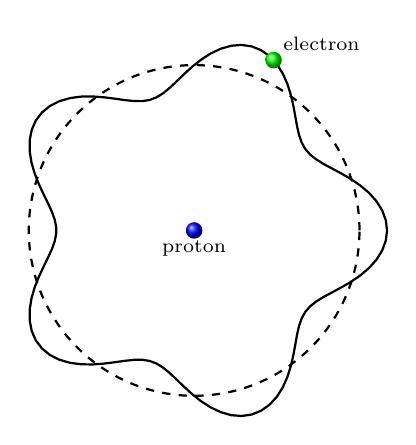
\begin{tikzpicture}[scale=0.7]
	\draw[thick,domain=0:360,samples=120] plot (\x:{3+.5*cos(5*\x)});
	\draw[thick,dashed] (0,0) circle (3);
	\shade [ball color = blue] (0,0) circle (0.15) node[below]{\scriptsize proton};
	\shade [ball color = green] (65:3.4096) circle (0.15) node[above right]{\scriptsize electron};
	\end{tikzpicture}
	
	\caption{the hydrogen atom}
\end{marginfigure}

electrostatic attraction by proton provides centripetal force for electron to move in circles



{
	
	\centering
	
	$\frac{e^2}{\ec r^2} = \frac{m_e v^2}{r} \RA v^2 = \frac{e^2}{\ec m_e r}$
	
}

for electron to \emph{constructively} superpose with itself, the perimeter of its orbit must be an integer multiple of its de Broglie wavelength

{
	
	\centering
	
	$2\pi r  = n \lambda \RA 2\pi r = \frac{nh}{m_e v} \RA v = \frac{nh}{2\pi m_e r}$
	
}

\noindent where $n$ is positive integer $1,2,3,\cdots$

compare the two equations, we can eliminate $v$

{
	
	\centering
	
	$\frac{e^2}{\ec m_e r} = \frac{n^2 h^2}{4\pi^2 m_e^2 r^2}$
	
}

we hence find radius of allowed orbits satisfies:

{
	
	\centering
	
	$\boxed{r_n = n^2 a_0} \quad \text{where }\, a_0 = \frac{h^2 \epsilon_0}{\pi m_e e^2} \approx 5.29 \times 10^{-11} \text{ m}$
	
}

\noindent so we see all allowed orbits must have a radius equal to integer multiple of $a_0$

total energy possessed by the electron consist of K.E. and electric P.E.:

{
	
	\centering
	
	$E = E_k + E_p = \frac{1}{2}m_e v^2 - \frac{e^2}{\ec r} = \frac{1}{2}m_e \frac{e^2}{\ec m_e r} - \frac{e^2}{\ec r} \RA E = -\frac{e^2}{8\pi\epsilon_0 r}$
	
}

substitute the allowed orbital radius, we find an expression for electron energy:

{
	
	\centering
	
	\begin{empheq}[box=\tcbhighmath]{equation*}{E_n = -\frac{R_E}{n^2}} \end{empheq} $\text{where }\, R_E = \frac{m_e e^4}{8 h^2 \epsilon_0^2} \approx 2.18\times10^{-18} \text{ J} \approx 13.6 \text{ eV}$
	
}

this shows electron can only have specific energies in the hydrogen atom



\subsection{electron energy levels}

it can be shown that for any atom, electrons can only have certain fixed values of energy

we say energy of electrons in an atom is \emph{discrete}, or \keypoint{quantised}

these allowed values of energies are called \keypoint{energy levels}\index{energy level}\footnote{If you study chemistry, you shall recall this idea of discrete energy levels is related to the concepts of energy shells and sub-shells of atoms.}

\begin{marginfigure}
	\centering
	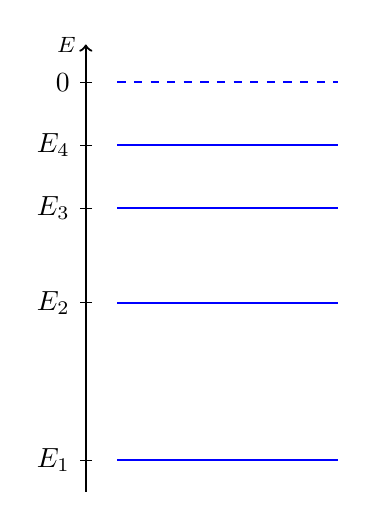
\begin{tikzpicture}[yscale=0.8,xscale=0.8]
	\foreach \s in {-6,-3.5,-2,-1}
	\draw[thick,blue] (0.5,\s) -- ++ (3.5,0);
	\draw[thick,blue,dashed] (0.5,0) -- ++ (3.5,0);
	\draw[thick,->] (0,-6.5) -- (0,0.6) node[left]{\footnotesize{$E$}};
	\draw(0.1,-6) --++ (-0.2,0) node[left]{$E_1$};
	\draw(0.1,-3.5) --++ (-0.2,0) node[left]{$E_2$};
	\draw(0.1,-2) --++ (-0.2,0) node[left]{$E_3$};
	\draw(0.1,-1) --++ (-0.2,0) node[left]{$E_4$};
	\draw(0.1,0) --++ (-0.2,0) node[left]{$0$};
	\end{tikzpicture}
	
	\caption{electron energy levels of some atom}		
\end{marginfigure}

\cmt \emph{quantisation} means an electron can have only specific values of energy in an atom

no intermediate value between levels is allowed

\cmt the lowest energy level is called the \keypoint{ground state}

any level higher than the ground state is called an \keypoint{excited state}

in our illustration, $E_1$ is the ground state, while $E_2$, $E_3$, $E_4$ are all excited states

\cmt electron energy levels are all \emph{negative}

to pull an electron away from the nucleus, work must be done to overcome electrostatic attraction

an electron at infinity would have greatest P.E., which is defined to be zero 

so orbiting electrons have energies less than zero

an electron that has zero energy would become a \emph{free} electron

\cmt electrons can jump, or \emph{transit}, between energy levels

electron transition is associated with emission or absorption of photon with the right energy



\begin{figure}[ht]
	\centering
	\begin{minipage}{0.48\textwidth}
		\begin{center}
			\begin{tikzpicture}[yscale=0.85,xscale=1]
			\foreach \s in {7,3,1.2,0.5,0.15}
			\draw[thick,blue] (0,-\s) -- ++ (4,0);
			\draw[thick,->] (-1,-7.5) -- (-1,0.2) node[left]{\footnotesize{$E$}};
			\draw[red,thick,->] (0.8,-3) node{$\bullet$} -- (0.8,-7);
			\draw[red,thick,->] (2.1,-1.2) node{$\bullet$} -- (2.1,-7);
			\draw [->, thick, purple, decorate, decoration={snake,post=lineto, post length=2mm}] (0.8,-5.6) --++ (2.4,0) ;
			\draw [->, thick, purple, decorate, decoration={snake,post=lineto, post length=2mm}] (2.1,-4) -- (3.8,-4);
			\node[twoline] at (3.6,-4.8) {photon\\emitted};
			\end{tikzpicture}
		\end{center}
	\end{minipage}\hfil
	\begin{minipage}{0.48\textwidth}
		\begin{center}
			\begin{tikzpicture}[yscale=0.85,xscale=1]
			\foreach \s in {7,3,1.2,0.5,0.15}
			\draw[thick,blue] (0,-\s) -- ++ (4,0);
			\draw[thick,->] (-1,-7.5) -- (-1,0.2) node[left]{\footnotesize{$E$}};
			\draw[red,thick,<-] (1.4,-3) -- (1.4,-7) node{$\bullet$};
			\draw [->, thick, purple, decorate, decoration={snake,post=lineto, post length=2mm}] (0,-5) -- (1.4,-5) ;
			\draw [->, thick, purple, decorate, decoration={snake,post=lineto, post length=2mm}] (0.3,-4) -- (3.6,-4);
			\node[twoline] at (3.5, -4.8){photon not\\absorbed};
			\node[twoline] at (0.5,-5.8){photon\\absorbed};
			\end{tikzpicture}
		\end{center}
	\end{minipage}
	
	\caption{emission and absorption of photons as a result of electron transitions}
\end{figure}


\subsection{atomic spectrum}



passing light through a \emph{prism} or a \emph{diffraction grating}, different wavelengths are separated, a pheonomenon known as \keypoint{dispersion}\index{dispersion}, this produces a \keypoint{spectrum}\index{spectrum} which shows distribution of energy emitted from the source in order of wavelengths

for example, white light consists of a range of wavelengths from around 400 nm to 700 nm, so it gives a \emph{continuous spectrum} with rainbow of colours

\begin{center}
	\pgfdeclareverticalshading{rainbow}{100bp}
	{color(0bp)=(Red); color(25bp)=(Red); color(30bp)=(OrangeRed); color(35bp)=(Orange); color(40bp)=(Gold); color(45bp)=(Yellow); color(50bp)=(GreenYellow); color(55bp)=(LimeGreen); color(60bp)=(Teal); color(65bp)=(DarkBlue); color(70bp)=(Indigo); color(75bp)=(Purple); color(100bp)=(Purple)}
	
\begin{tikzpicture}[shading=rainbow]
	\shade[shading angle=90] (0,0) rectangle (12,2);
	\end{tikzpicture}
	
	continuous spectrum of white light
\end{center}

electron transition between different levels causes emission or absorption of photons

this leads to the emission spectrum and absorption spectrum of atoms

\subsection*{emission spectrum}

\emph{hot gases} of an element can release photons, giving an \keypoint{emission spectrum}\index{spectrum!emission spectrum}

this happens when an electron transits from a high energy level to a lower level

energy of the photon emitted is equal to energy difference between the two levels

since electron energy levels are discrete, only specific changes of energies are possible, so only photons with specific energies can be emitted

this means photons emitted only have specific wavelengths, or specific frequencies

so a collection of sharp and bright lines are seen in emission spectrum

\begin{figure*}[ht]
	\centering
	
\begin{tikzpicture}
	\draw [fill] (0,0) rectangle (12,2);
	\draw [ultra thick, orange] (11,0) -- (11,2);
	\draw [ultra thick, yellow] (9,0) -- (9,2);
	\draw [ultra thick, green] (3.5,0) -- (3.5,2);
	\draw [ultra thick, blue] (2,0) -- (2,2);
	\end{tikzpicture}
	
	\caption{emission spectrum of the hydrogen atom}
\end{figure*}

\cmt emission spectrum is a \emph{discrete} spectrum, also called a \emph{line} spectrum

\cmt atoms of each element has a unique electron energy level structure

so each element produces a unique emission spectrum, leading to quite a few applications:

\begin{compactitem}
	\item[-] explains the colour of flames when a particular chemical element is present
	
	\item[-] allows the identification of elements in an unknown substance in chemical analysis
	
	\item[-] explains varied colours of electric signs lighted by gas-discharge tubes
\end{compactitem}


\subsection*{absorption spectrum}


pass white light through a \emph{cool gas}, photons with the right energies can be absorbed, giving rise to an \keypoint{absorption line spectrum}\index{spectrum!absorption spectrum}

by absorbing photon, electron can transit from a low energy level to a higher level

energy of the photon absorbed must equal energy difference between the two levels

since electron energy levels are discrete, so only photons with specific energies can be absorbed, while other photons are unaffected as they pass through the gas

wavelengths of these absorbed photons will be missing in the emergent spectrum

so we would observe a set of \emph{dark lines} appearing in a background of continuous spectrum


\begin{figure}[ht]
	\centering
	
\begin{tikzpicture}[shading=rainbow]
	\shade[shading angle=90] (0,0) rectangle (12,2);
	\foreach \x  in {1.9,4.4,5.9,7.6,8.2,9.9,11.4}
	\draw [very thick] (\x,0) -- (\x,2);
	\end{tikzpicture}
	\caption{absorption spectrum for some element}
\end{figure}

\cmt absorption spectrum is also a \emph{discrete} spectrum, or a \emph{line} spectrum

\cmt as photons with the right energies are absorbed, they can be re-emitted through \emph{de-excitation}

but these photons are re-emitted in \emph{random} directions

so they would still appear dark compared with those unaffected wavelengths

\cmt absorption spectrum is widely used in many areas

\begin{compactitem}
	\item[-] determine the composition of a particular substance in analytical chemistry
	
	\item[-] determine chemical compositions of stars in astronomical spectroscopy
	
	\item[-] explain colour of chemicals in terms of the complementary colour of photons absorbed  
	
\end{compactitem}


%\vspace*{\baselineskip}

%for either emission or absorption process, energy of photon must match the difference between two electron energy levels: $\boxed{hf = E_\text{high} - E_\text{low}}$

\example{Some electron energy levels of the hydrogen atom is shown. Find the longest and the shortest wavelength produced by electron transitions between the energy levels given.}\label{ex-hydrogen}

\begin{figure}[ht]
	\centering
	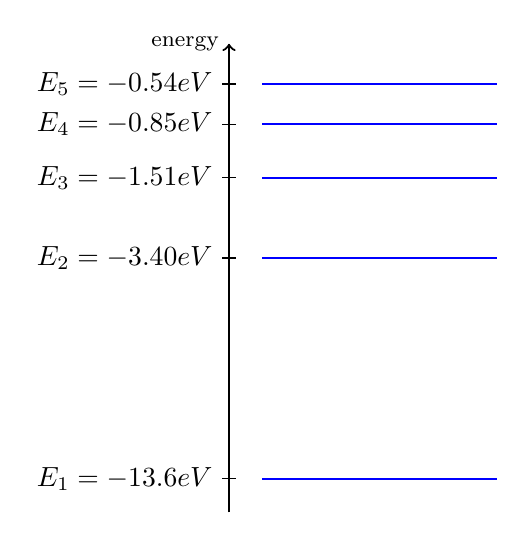
\begin{tikzpicture}[scale=0.85]
	\foreach \s in {-6,-2.7,-1.5,-0.7,-0.1}
	\draw[thick,blue] (0.5,\s) -- ++ (3.5,0);
	\draw[thick,->] (0,-6.5) -- (0,0.5) node[left]{\footnotesize{energy}};
	\draw(0.1,-6) --++ (-0.2,0) node[left]{$E_1=-13.6 \text{ eV}$};
	\draw(0.1,-2.7) --++ (-0.2,0) node[left]{$E_2=-3.40 \text{ eV}$};
	\draw(0.1,-1.5) --++ (-0.2,0) node[left]{$E_3=-1.51 \text{ eV}$};
	\draw(0.1,-0.7) --++ (-0.2,0) node[left]{$E_4=-0.85 \text{ eV}$};
	\draw(0.1,-0.1) --++ (-0.2,0) node[left]{$E_5=-0.54 \text{ eV}$};
	\end{tikzpicture}		
	
	\caption{energy levels of the hydrogen atom}
\end{figure}

\begin{soln} energy of photon emitted equals change of electron energy level: $\frac{hc}{\lambda} = \Delta E$, or $\lambda = \frac{hc}{\Delta E}$

transition with least/greatest energy change gives rise to longest/shortest wavelength, so

\eqskip $E_5 \to E_4 \ra \lambda_\tmax = \frac{hc}{E_5-E_4} = \frac{6.63\times10^{-34}\times3.0\times10^8}{(0.85-0.54)\times1.60\times10^{-19}} \approx 4.0\times10^{-6} \text{ m} \quad$ (infra-red)
	
\eqyskip 
	
\eqskip $E_5 \to E_1 \ra  \lambda_\tmin = \frac{hc}{E_5-E_1} = \frac{6.63\times10^{-34}\times3.0\times10^8}{(13.6-0.54)\times1.60\times10^{-19}} \approx 9.5\times10^{-8} \text{ m} \quad$ (ultraviolet) \end{soln}
	

\example{The emission spectrum of the hydrogen atom consists of a number of wavelengths in the visible spectrum. Given that the visible spectrum consists of light of wavelengths within the range from 380 nm to 740 nm, also use data in Example \ref{ex-hydrogen}, find the energies of visible photons that can be produced by transitions between the energy levels shown.}\sidenote{The H$_\alpha$ line is the brightest hydrogen line in the visible range. It plays an important role in astronomy, as it can be used to study a star's surface temperature, the velocity of a distant stellar object, etc.}

\begin{soln} let's first find the range of energies, in eV, for visible photons

\eqskip $E_\tmax = \frac{hc}{\lambda_\tmin} = \frac{6.63\times10^{-34}\times 3.0 \times10^8}{380\times10^{-9}} \approx 5.23\times10^{-19} \text{ J} = \frac{5.23\times10^{-19}}{1.60\times10^{-19}} \text{ eV} \approx 3.27 \text{ eV}$
 $E_\tmin = \frac{hc}{\lambda_\tmax} = \frac{6.63\times10^{-34}\times 3.0 \times10^8}{740\times10^{-9}} \approx 2.69\times10^{-19} \text{ J} = \frac{2.69\times10^{-19}}{1.60\times10^{-19}} \text{ eV} \approx 1.68 \text{ eV}$

we shall find the combinations of electron energy levels such that their difference fall within the range between 1.68 eV and 3.27 eV, by trial and error, we find three possible combinations:

\begin{compactenum}
	\item[(1)] $E_3 \to E_2 \ra 3.40 - 1.51 = 1.89 \text{ eV}$
	
	\item[(2)] $E_4 \to E_2 \ra 3.40 - 0.85 = 2.55 \text{ eV}$
	
	\item[(3)] $E_5 \to E_2 \ra 3.40 - 0.85 = 2.85 \text{ eV}$
\end{compactenum}

these emisssion lines are called H$_\alpha$ (656 nm), H$_\beta$ (486 nm) and H$_\gamma$ (435 nm) lines

they are three of the four the hydrogen emission lines that are visible to human eyes \end{soln}\sidenote{These lines belong to a family of the spectral lines of the hydrogen atom, known as the \emph{Balmer lines}, named after Johann Balmer. Balmer discovered an empirical equation to predict the series in 1885, but the reason why the equation worked was eventually clarified by Neils Bohr with the atomic model which now bears his name. We now understand the Balmer lines correspond to emissions of photons by electrons jumping to the second level from higher energy states.}



\example{A white light is incident on a cloud of cool hydrogen gas. In the emergent spectrum, a dark line is observed at a wavelength of 435 nm. Determine the energy change that gives rise to this dark line.}

\begin{soln}
    
 photon absorbed: $E = \frac{hc}{\lambda} = \frac{6.63\times10^{-34}\times 3.0 \times10^8}{435\times10^{-9}} \approx 4.57\times10^{-19} \text{ J} = \frac{4.57\times10^{-19}}{1.60\times10^{-19}} \text{ eV} \approx 2.86 \text{ eV}$

note that $3.40 - 0.54 = 2.86 \text{ eV}$, so this dark line is due to the electron transition: $E_2 \to E_5$ \end{soln}

\question{If we only consider the electron energy levels given in Example \ref{ex-hydrogen}, how many different wavelengths can be detected in the emission spectrum of the hydrogen atom ?}

\question{Three lines are observed at wavelengths 486 nm , 656 nm, and 1880 nm in the emission spectrum of hydrogen atoms. (a) Calculate the photon energies for these wavelengths. (b) Draw a diagram with \emph{three} labelled energy levels, and show the energy changes for the three wavelengths produced with arrows in your diagram.}

\begin{marginfigure}
	\centering
	\vspace*{-25pt}
	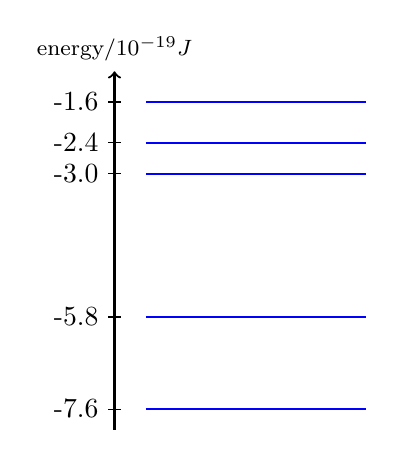
\begin{tikzpicture}[xscale=0.8, yscale=0.65]
	\foreach \s in {-7.6,-5.8,-3.0,-2.4,-1.6} {
	\draw[thick,blue] (0.5,\s) -- ++ (3.5,0);
	\draw(0.1,\s) --++ (-0.2,0) node[left] {\s};
	}
	\draw[thick,->] (0,-8) -- (0,-1) node[above]{\footnotesize{energy/$10^{-19}\text{ J}$}};	
	\end{tikzpicture}		
	
	\caption{energy levels of the helium atom}
	\vspace*{-15pt}
\end{marginfigure}

\question{The relative cool atmosphere of the sun could give rise to dark lines in the spectrum of sunlight.	One particular dark spectral line has a wavelength of 590 nm. By reference to the energy levels of the helium atom, suggest how this dark line provides evidence of the presence of helium in sun's atmosphere. You may draw an arrow to show the possible electron transition that gives rise to this dark line.}



\subsection{band theory}

\subsection{energy bands}

in an isolated atom, electrons have discrete energy levels 

in solids, interaction between neighbouring atoms causes change of energies

original energy levels split into a band with many sub-levels

number of sub-levels in each band equals number of atoms in solid in general

due to very large number of atoms, sub-levels (seem to) form \emph{continuous} \keypoint{energy bands}\index{energy band}

\begin{figure}[htp]
	\centering
	\begin{tikzpicture}[yscale=0.56,xscale=.8]
	\foreach \s in {0,1.5,3.5,7}{
		\draw[thick,blue] (0,-\s) -- ++ (3.6,0);
		\foreach \step in {-0.4,-0.3,...,0.4}	\draw[thick,blue] (6,-\s+\step) -- ++ (3.6,0) ;
		\draw[thick,blue,fill=blue!30] (12,-\s-0.5) rectangle (15.6,-\s+0.5);
	}
	\draw[thick,->] (-.8,-8) -- (-.8,1) node[left]{$E$};
	\node[below,twolinecap] at (1.8,-9) {dicrete energy levels\\in isolated atom};
	\node[below,twolinecap] at (7.8,-9) {split energy sub-levels\\due to interactions};
	\node[below,twolinecap] at (13.8,-9) {energy bands formed\\in many-particle system};
	\end{tikzpicture}
\end{figure}

\begin{marginfigure}
	\vspace*{0pt}
	\centering
	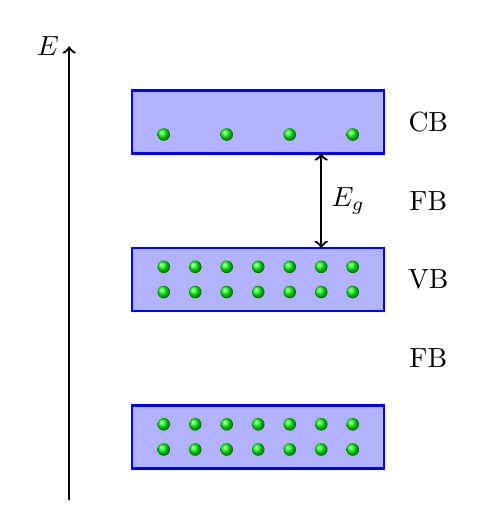
\begin{tikzpicture}[scale=0.8]
	\draw[thick,->] (-1,-0.5) --++ (0,7.2) node[left]{$E$};
	\foreach \s in {0,2.5,5}
	\draw[thick,blue,fill=blue!30] (0,\s) rectangle (4,\s+1);
	\foreach \x in {0.5,1,...,3.5} \foreach \y in {0.3,0.7,2.8,3.2}
	\shade [ball color = green] (\x,\y) circle (0.1); 
	\foreach \x in {0.5,1.5,2.5,3.5} \shade [ball color = green] (\x,5.3) circle (0.1); 
	\node at (4.7,5.5) {CB};
	\node at (4.7,3) {VB};
	\node at (4.7,4.25) {FB};
	\node at (4.7,1.75) {FB};
	\draw[thick,<->] (3,3.5) -- (3,5) node[midway,right]{$E_g$};
	\end{tikzpicture}
	\vspace*{-12pt}
\end{marginfigure}

in solids, electrons fill up from lowest energy bands available (see figure for a rough idea)


\keypoint{forbidden bands}\index{energy band!forbidden band} (FB) represent energies that electrons are not allowed to take



highest fully filled band is called \keypoint{valence band}\index{energy band!valence band} (VB)

next partially filled or empty band is called \keypoint{conduction band}\index{energy band!conduction band} (CB)

separation between valence band and conduction band defines \keypoint{band gap}\index{energy band!band gap} ($E_g$) of material 


\subsection{band theory \& electrical conductivity}\label{band-theory}

electrical conductivity of material can be explained by its band structure

low-energy bands below VB are usually fully filled at all times, all states are occupied, electrons cannot move freely to form electric currents, so we are not interested in low-energy bands

conductivity of material will depend on whether there are free \emph{charge carriers} in CB and VB


\subsection*{metallic conductors}

for typical metals, CB \emph{overlaps} with VB, i.e., there is no band gap

there exist vacant states for conduction electrons to occupy at ease

this means conduction electrons are free to move around to form currents

as temperature rises, there is no significant change in number of free electrons

but \emph{lattice vibration} of atoms increases, electrons become more likely to collide with vibrating atoms, so resistance of metal increases with temperature

\cmt metals are \emph{opaque} to visible light or other low-frequency radiation

width of CB for a typical metal is about $2\sim3 \text{ eV}$

low-energy photons can be absorbed by conduction electrons

visible light, infra-red, microwave therefore cannot pass through metal

\cmt metals are \emph{transparent} to high-frequency radiation such as X-rays

if X-ray photons were absorbed, electrons would take energies in forbidden band

but this is not allowed, so high-frequency photons penetrate through metal

\subsection*{insulators}

\begin{marginfigure}
	\vspace*{-5pt}
	\centering
	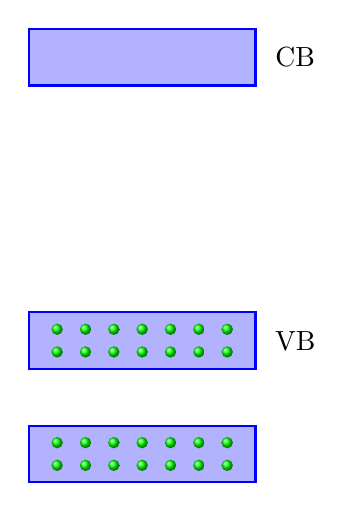
\begin{tikzpicture}[scale=0.72]
	\foreach \s in {0,2,7}
	\draw[thick,blue,fill=blue!30] (0,\s) rectangle (4,\s+1);
	\foreach \x in {0.5,1,...,3.5} \foreach \y in {0.3,0.7,2.3,2.7}
	\shade [ball color = green] (\x,\y) circle (0.1); 
	\node at (4.7,7.5) {CB};
	\node at (4.7,2.5) {VB};
	\end{tikzpicture}
	
	band structure of insulator
\end{marginfigure}

examples of insulators include glass, diamond, etc.

in normal conditions, CB of insulator is empty, energy bands up to VB are fully filled, so no movement of electron is possible, material has poor conductivity

insulators also have huge band gap\footnote{To be a little more precise, materials with a band gap $E_g \approx 5$ eV or greater are regarded as insulators.}\footnote{There exist a class of insulators called \emph{Mott insulators} which do not have large band gaps. Their poor conductivity at low temperatures is due to electron-electron interactions, which are not considered under conventional band theories.}, so thermal excitations cannot easily make VB electrons jump into CB

insulators remain poor conductors as temperature rises



\question{Diamond has a band gap $E_g \approx 6.0 \text{ eV}$. By reference to its electronic band structure, explain why diamond appears \emph{transparent} to visible light?}

\subsection*{intrinsic semiconductors}

examples of an intrinsic semiconductor are silicon and germanium

band structure of an intrinsic semiconductor is similar to that of insulators

at low temperature, no free electron from the empty CB and completely occupied VB, so semi-conductors are not conductive in normal conditions

however, semiconductors have much narrower band gaps

as temperature rises, VB electrons gain thermal energy to cross band gap and enter CB

the electrons jumped into CB surely can move around to form electric currents

at the same time, VB is no longer completely filled, \emph{holes} are formed

a hole is a site where an electron is missing, neighbouring electrons can move to fill the hole and leave a new hole, but this can be thought of as the hole moving about

there are now more \emph{charge carriers} (negatively-charge electrons and positively-charged holes) available, so semiconductor has better conductivity, resistance of material would decrease

\begin{figure}[ht]
	\centering
	\begin{tikzpicture}[scale=1]
	\foreach \s in {0,2,4}
	{
		\draw[thick,blue,fill=blue!30] (0,\s) rectangle (4,\s+1);
		\foreach \x in {0.5,1,...,3.5} \foreach \y in {0.3,0.7,2.3,2.7}
		\shade [ball color = green] (\x,\y) circle (0.1); 
		\draw[thick,blue,fill=blue!30] (7,\s) rectangle (11,\s+1);
		\foreach \x in {0.5,1,...,3.5} \foreach \y in {0.3,0.7,2.3}
		\shade [ball color = green] (\x+7,\y) circle (0.1);
	}
	\foreach \x in {0.5,1,2,2.5,3.5} \shade [ball color = green] (\x+7,2.7) circle (0.1);
	\draw [very thick,dashed,red] (8.5,2.7) circle(0.2);
	\draw [very thick,dashed,red] (10,2.7) circle(0.2);
	\shade [ball color = green] (8.5,4.3) circle (0.1);
	\shade [ball color = green] (10,4.3) circle (0.1);
	\draw[thick,red,->] (8.5,2.7)++(120:0.2) [out=120, in=250] to ++(0.05,1.3);
	\draw[thick,red,->] (10,2.7)++(60:0.2) [out=60, in=290] to ++(-0.05,1.3);
	\node at (4.5,4.5) {CB};
	\node at (4.5,2.5) {VB};
	\node at (11.5,4.5) {CB};
	\node at (11.5,2.5) {VB};
	\node[twolinecap] at (2,-1) {band structure of an intrinsic\\semiconductor at low temperature};
	\node[twolinecap] at (9,-1) {at higher temperature VB electrons\\cross band gap and enter CB};
	
	\end{tikzpicture}
\end{figure}

\cmt \emph{lattice vibration} could also affect resistance of semiconductors

as temperature rises, vibration of atoms increases, charge carrier are more likely to get scattered, causing a decrease in conductivity

but the effect of more charge carriers is far greater than effect due to lattice vibration

so resistance of semiconductor decreases at higher temperature

\example{Silicon has a band gap $E_g \approx 1.1 \text{ eV}$. State and explain whether it becomes conducting when exposed to red light of $600 \text{ nm}$.}

\begin{soln}
    
 energy of radiation: $E=\frac{hc}{\lambda} = \frac{6.63\times10^{-34}\times3.0\times10^8}{600\times10^{-9}} \approx 3.32\times10^{-19} \text{ J} \approx 2.1 \text{ eV} > E_g$

this energy is sufficient to make valence electrons in silicon to cross band gap

silicon now possesses conducting electrons and holes therefore becomes conducting \end{soln}

\question{Use band theory to explain why an LDR (light-dependent resistor) has a very high resistance in the dark, but its resistance drops dramatically when being exposed to light.}



